\chapter{Degeneration}
Innerhalb dieses Kapitels wird der Ansatz der \textit{Degeneration} vorgestellt.

Die Benennung schöpft sich aus der Nähe zu genetischen Algorithmen \todo{genauer, was das ist?}, allerdings aus einer invertierten Perspektive: Um auf unbekannte Modelle einzugehen, wird hierbei von einem korrekt erkannten Bild \textit{weggearbeitet}.

~\newline Zunächst wird das Konzept anhand von Pseudocode genauer erläutert. Anschließend wird die Implementierung des Algorithmus für die Verwendung der unbekannten Trasi-AI vorgestellt, und den Abschluss dieses Kapitels bildet eine lokale Implementierung zuzüglich einiger Verbesserungen, welche sich aufgrund der Limitierungen des Zugriffes auf die \textit{remote-AI} nicht angeboten haben.
\section{Konzept}
Die Grundlegende Idee des Algorithmus bezieht sich darauf, ein Urbild $i$ zu einem Abbild $\hat{i}$ zu manipulieren, welches von dem unbekannten Klassifizierungsalgorithmus weiterhin korrekt erkannt wird. 

~\newline Abhängig von der Stärke der Manipulation soll eine $Tiefe$ gewählt werden, ab welcher der Algorithmus beendet wird. Als Beispiele der Manipulation seien insbesondere Rauschen und Glätten genannt, allerdings auch Kantenschärfung und Veränderungen der Helligkeit und anderer Metaparameter. 

~\newline Mit fortschreitender Tiefe wird nahezu jedes Bild unkenntlich. Zusätzlich sollten allerdings weitere Parameter als Abbruchkriterien aufgenommen werden, konkret eine Anzahl an Gesamt-Iterationen und ein Abbruch, sollten keine weiteren Fortschritte erreicht werden.

\newpage
\paragraph{Pseudocode} ~\newline 
Folgende Parameter erwartet unsere (generische) Implementierung des Degeneration-Algorithmus: 
\begin{itemize}
	\item Einen Eingabewert $i$
	\item Eine Manipulations-Funktion $a : i \rightarrow \hat{i}$
	\item Eine Klassifizierungsfunktion $p : i \rightarrow \mathrm{R}$
	\item Eine gewünschte Tiefe $d$ (empfohlen, nicht notwendig)
	\item Eine Iterationszahl $its$ (empfohlen, nicht notwendig)
	\item Ein Schwellwert $t$ , um wie viel \% die Vorhersage schlechter sein darf, als das vorhergegangene Bild 
\end{itemize}
Auf einige der Punkte wird in den Anmerkungen gesondert eingegangen. ~\newline
\IncMargin{1em}
\begin{algorithm}
	\SetKwInOut{Input}{input}
	\SetKwInOut{Output}{output}
	\Input{i,a,p,d,its,t}
	\Output{$\hat{i}$, score}
	\BlankLine
	$depth  \leftarrow 0$, $loop \leftarrow0$ \;
	$s \leftarrow p(i)$\;
	$ii \leftarrow i , is \leftarrow s$ \;
	\While{$depth<d ~ || ~ loop <its$}{
		$ai \leftarrow a(i)$ \;
		$as \leftarrow p(ai)$ \;
		\If{$as >= is-t$}{
			$is \leftarrow as$\;
			$ii \leftarrow ai$\;
			depth++\;
		}
		loop ++\;
	}
	return ii,is\;
	
	\caption{Degeneration}\label{algo_degen}
\end{algorithm}\DecMargin{1em}
\newpage
\paragraph{Anmerkungen}~\newline 
Die Manipulationsfunktionen müssen genau ein Bild der Größe (x,y) erhalten und genau ein Bild der Größe (x,y) wiedergeben, und (für die generischen Implementierungen) keine weiteren Parameter erhalten. 

Zusätzlich sollte die Manipulationsfunktion zufällige Elemente erhalten. Sollte eine einfache,idempotente Glättungsfunktion den Schwellwert nicht erfüllen, so wird niemals eine größere Tiefe erreicht.  

~\newline Tiefe, Schwellwert und Manipulationsfunktion müssen aufeinander abgestimmt werden. Es gibt einige Funktionen, welche eine starke Veränderung hervorrufen, und für welche eine geringe Tiefe bereits ausreicht. Auf der anderen Seite dieses Spektrums können Funktionen, welche lediglich minimale Änderungen vornehmen, schnell große Tiefen erreichen, ohne ein merklich verändertes Bild hervorgerufen zu haben. 

Diese Parameter auszubalancieren obliegt dem Nutzer. 

Bei der Auswahl der Parameter sollte zusätzlich überschlagen werden, wie groß die letztendliche Konfidenz ist, falls die maximale Tiefe erreicht wird. 

~\newline Innerhalb der Implementierungen sollte zusätzlich eine \textit{verbose}-Funktion eingebaut werden. Hiermit kann zum einen ein ergebnisloser Versuch frühzeitig erkannt werden, und zusätzlich, ob der Algorithmus sich festgefahren hat. Üblicherweise kann man erkennen, wenn die Manipulationsfunktion \textit{zu stark} ist (bzw. der Schwellwert zu niedrig gewählt wurde).

~\newline Der oben genannte Algorithmus lässt sich auch für Text- oder Sprach-basierte Klassifikationen adaptieren. 

Hierfür müssen lediglich andere Manipulations- und Klassifizierungs-Funktionen gewählt werden.
\newpage
\section{Implementierung Remote}
Im Rahmen des Wettbewerbs wurde mit einer Rest-API \todo{Marker nach oben} gearbeitet, welche besondere Herausforderungen mit sich bringt: 

\begin{itemize}
	\item Anfragen können fehlschlagen
	\item zwischen Anfragen muss ein Timeout liegen
	\item Mehrere Nutzer, welche die API beanspruchen, blockieren sich
\end{itemize}
~\newline
Zusätzlich wurde der Grundalgorithmus um die \textit{Verbose}-Funktion und eine History erweitert. Mithilfe der \textit{History} können anschließend hilfreiche Plots erstellt werden. 

Diese wurden für den untenstehenden Code weggelassen.
~\newline~\newline
Ebenso ist anzumerken, das ignoriert wurde, welche Klasse zuerst erzeugt wurde. Solange irgendeine Klasse mit einer passenden Konfidenz gefunden wurde, wird dies als hinreichend erachtet. Im Normalfall bleibt es allerdings bei derselben Klasse. 

~\newline 
Die Klassifizierungsfunktion wird innerhalb der Remote-Degeneration durch einige Hilfsfunktionen umgesetzt. Diese bereiten ein als \textit{Bytearray} vorliegendes Bild entsprechend auf und senden es an das Trasi-Webinterface (Die Methode \textit{Scorer.Send\_ppm\_image(img)}) und gibt ein JSON-Array der Scores wieder. 

Die Hilfsmethode \textit{Scorer.get\_best\_score(response)} gibt den höchsten gefunden Score wieder.
\newpage
\begin{small}
\improvement{Zeilennummern, Caption}
\pythonexternal{CodeSnippets/remoteDegenerationSnippet.py}
\end{small}
\section{Ergebnisse Remote}
In diesem Abschnitt werden die mit der Degeneration erzielten Ergebnisse in Bezug auf die Trasi-Schnittstelle vorgestellt. Zunächst werden einige positive Beispiele (Erfolge) gezeigt, anschließend einige Probleme die aufgetreten sind und zuletzt noch ein kurzes Zwischenfazit gezogen. 
\paragraph{Positive Ergebnisse} ~\newline Die zuverlässigsten Ergebnisse wurden mit einfachem Rauschen erzeugt. Die Abbildung \ref{fig:stoptiefe600} zeigt, dass zunächst vorallem die Pixel außerhalb des eigentlichen Schildes verändert werden - ein erwartetes verhalten. Die farbstarken bunten Pixel sind hierbei entstanden, da Werte welche die gültige Reichweite [0,255] verlassen, wieder zyklisch zurück in den Farbbereich geholt werden. Sollte ein Farbwert durch das Rauschen einen Wert -2 erreichen, wird er auf 253 gesetzt.  

\begin{figure}[h]
	\centering
	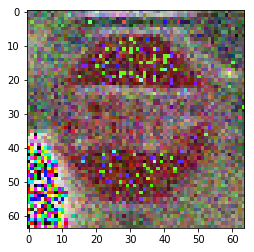
\includegraphics[width=0.4\linewidth]{Images/DegenSamples/StopTiefe600}
	\caption[Degeneration Tiefe 600]{Rausch - Degeneration mit 600 Iterationen}
	\label{fig:stoptiefe600}
\end{figure}

Während die Abbildung \ref{fig:stoptiefe600} noch als Verkehrsschild zu erkennen ist, führt ein längeres ausführen der Degeneration zu einem Ergebniss wie in Abbildung \ref{fig:stoptiefe4000}. Um dieses Ergebnis zu erzielen wurden 4400 sekunden benötigt, also ca. 73 Minuten.

\begin{figure}[h]
	\centering
	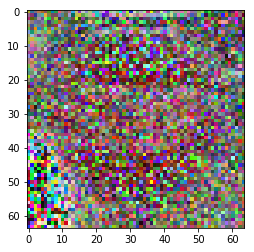
\includegraphics[width=0.4\linewidth]{Images/DegenSamples/StopTiefe4000}
	\caption[Degeneration Tiefe 4000]{Rausch - Degeneration mit 4000 Iterationen}
	\label{fig:stoptiefe4000}
\end{figure}

Die Plots in Abbildung \ref{fig:plotTiefe4000} stellen den Verlauf des Algorithmus dar: Das erste Diagramm zeigt einen Verlauf der aktuellen \textit{Tiefe} über die Iterationen dar, der zweite die jeweils produzierten Genauigkeit der jeweiligen Iteration (nicht nur die der akkzeptierten), und der letzte Plot visualisiert diejenigen Iterationen, an welchen eine Änderung stattgefunden hat (weißer Strich) oder keine (schwarzer Strich). Innerhalb der Implementierung werden ebenfalls standartmäßig diese Plots erzeugt.

\begin{figure}[h]
	\centering
	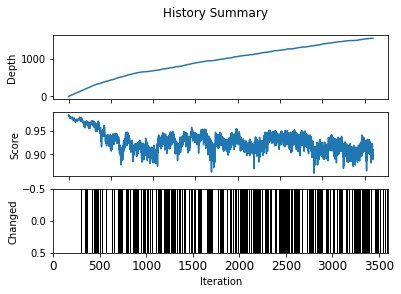
\includegraphics[width=0.6\linewidth]{Images/DegenSamples/StopTiefe4000Plot}
	\caption[Plot Degeneration]{Plot der Rausch-Degeneration}
	\label{fig:plotTiefe4000}
\end{figure}
~\newline Es wurden ebenfalls einige sehr positive Ergebnisse mit einer Mischung aus starkem Rauschen und Glätten erzeugt, allerdings waren diese nicht zuverlässig reproduzierbar. 

\paragraph{Negative Ergebnisse} ~\newline Es gab zwei primäre Fehlerquellen in Bezug auf die Remote-Degeneration: Die Auswahl von Bildern, welche im GTSRB-\textit{Training}-Set waren, sowie die Auswahl ungeeigneter Manipulationsfunktionen. 
~\newline
Die AI innerhalb der Schnittstelle scheint sich die Bilder aus dem Trainingsset \textit{gemerkt} zu haben. Bereits minimale, unwichtige Änderungen des Schildes (z.B. einfügen einiger blauer Punkte im Hintergrund) führen zu einer drastischen Verschlechterung des Ergebnisses. Dieses starke \textit{Ausschlagen} des Scores machte die Benutzung der Degeneration unbrauchbar.
\begin{figure}[h]
	\centering
	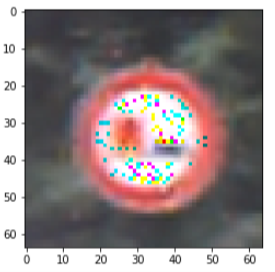
\includegraphics[width=0.5\linewidth]{Images/DegenSamples/OverFitSmaller}
	\caption[Degeneration overfit]{Rausch-Degeneration auf Trainingsbild - 36000 Iterationen}
	\label{fig:DegenOverfit}
\end{figure}
~\newline
Dieses Problem hat sich herauskristallisiert, als über einen längeren Zeitraum (\~ 10 Stunden) kein Bild erzeugt wurde, welches auch nur leicht verändert wurde. Die einzigen Änderungen, welche erzielt wurden, waren innerhalb des weißen Bereiches des Überholverbotsschildes wie in Abbildung \ref{fig:DegenOverfit}. Es wurden aber ebenfalls keine Änderungen vorgenommen außerhalb des Schildes, wo diese zu erwarten wären und bei vorhergehenden Versuchen auch zu beobachten waren (vgl. Abbildung \ref{fig:stoptiefe600}). 
~\newline
Dieses Problem tritt ausschließlich (allerdings zuverlässig) bei der Verwendung von Bildern aus dem Trainingsset auf. Es tritt nicht auf sobald man Bilder aus dem Test-Set verwendet oder \textit{GTSRB-fremde} Bilder (vorausgesetzt, sie besitzen eine akzeptable Startkonfidenz). 

Innerhalb der lokalen Implementierung ist dieses Problem ebenfalls aufgetreten, konnte allerdings behoben werden, sobald man das Overfitting erkannt hatte.
\paragraph{Fazit} ~\newline
Innerhalb dieses kurzen Zwischenfazits sollen noch einmal die Vor- und Nachteile der Degeneration zusammengefasst werden: ~\newline ~\newline  
\begin{tabular}{|p{7.5cm}|p{7.5cm}|}
	\hline 
	\textbf{Vorteile} & \textbf{Nachteile} \\ 
	\hline 
	\textbf{Model-Agnostic:} \newline Der Algorithmus funktioniert unabhängig und ohne Wissen über das zugrundeliegende Modell & \textbf{Zeitintensiv:} \newline v.A. die Remote-Variante benötigt größere Zeitspannen \\ 
	\hline 
	\textbf{Kontext-Unabhängig:} \newline Die Herangehensweise ist nicht auf Bilderkennungen limitiert & \textbf{Vorwissen benötigt:} \newline Der Sinn des zugrundeliegenden Models muss bekannt sein, und ein geeignetes Startbild muss ausgewählt werden  \\ 
	\hline 
	\textbf{Erweiterbar:} \newline Die Manipulationsfunktionen können weiter ausgebaut werden und haben noch großes Potenzial & Die Degeneration erzielt bei empfindlichen Modellen schlechter Ergebnisse - gerade \textit{professionelle} Modelle sollten lange brauchen, um so überlistet zu werden \\ 
	\hline 
	\textbf{Simpel:} \newline Der Algorithmus ist einfach implementiert und erläutert, er benötigt keine höhere Mathematik oder Vorwissen zur Thematik \textit{Machine Learning} und der Modelle/Verfahren im Speziellen & Im Remote-Umfeld kann die Degeneration als DDoS wahrgenommen werden und entsprechend frühzeitig unterbunden werden. \\ 
	\hline 
\end{tabular} \improvement{Caption und Label} ~\newline ~\newline
Als besonderen Fall sind solche Modelle zu nennen, die mit jeder Anfrage \textit{hinzulernen}: ~\newline Diese sind entweder besonders anfällig gegenüber der Degeneration, weil sie die bereits veränderten Bilder als \textit{korrekte} klassifizieren und somit den Entstehungsprozess der Degeneration verinnerlichen, oder sie \textit{härten} sich mit jedem Versuch gegen die neuen Änderungen und sind de facto immun gegen diesen Angriff.  

\todo{Solche Modelle sind selten im Einsatz, weil zuviel Schabernack damit getrieben werden kann. Hierfür brauche ich noch eine Quelle}
\section[Implementierung Lokal]{Implementierung Lokal \newline Anpassungen und Verbesserungen} 

Innerhalb dieses Abschnittes werden zunächst die Änderungen bei der lokalen Verwendung des Algorithmus kurz behandelt, und anschließend zwei konzeptionelle Verbesserungen vorgestellt: Parallel- und Batch-Varianten des Algorithmus. 

Auf weitere Code-Beispiele wird im Rahmen des Umfanges verzichtet - sie befinden sich im Anhang.

\paragraph{Anpassungen} ~\newline Für die lokale Implementierung wurde zunächst ein eigenes Modell (von Grund auf) trainiert mithilfe der GTSRB-Daten. Das \textit{Scoring} der Remote-Implementierung wird durch die \textit{predict()}-Funktion des Models ersetzt.

Als zusätzliche Erweiterung wurde für die lokale Implementierung umgesetzt, dass sich der Nutzer für eine bestimmte Klasse entscheiden kann, auf welche die Degeneration ausgelegt ist. Es wird also zuverlässig bspw. ein Stoppschild erzeugt, und kein beliebiges Schild mit hohem Score. 

~\newline Des Weiteren entfällt die Wartezeit, welche für die Schnittstelle benötigt wurde, sowie die Wartezeit. Letzteres erhöht die Geschwindigkeit des Algorithmus maßgeblich. 

~\newline Eine zusätzliche, passive Verbesserung wurde erzielt, indem die Verwendung der \textit{GPU-Acceleration} von Tensorflow eingebunden wurde \todo{Quelle? Oder Ausarbeiten?}. Diese beschleunigte nicht nur das Training des lokalen Models maßgeblich, sondern auch die Vorhersagen, insbesondere für die Batch-Variante, wurden um ein vielfaches ($\approx$Faktor 20) schneller.  

\paragraph{Fazit}~\newline Das wichtigste Fazit, welches im Umgang mit der lokalen Implementierung gezogen werden konnte, ist die nicht-verwendbarkeit der lokalen Bilder für die Schnittstelle. Während dies ursprünglich die Motivation war, schnell lokal Irrbilder zu erzeugen und Remote zu verwenden, stellte sich heraus das die lokalen Irrbilder keine guten Scores an der Schnittstelle erzielten und vice versa. 

~\newline Es ist anzunehmen, das die Modelle dieselben stärken haben (Verkehrsschilder korrekt zu erkennen), allerdings unterschiedliche \textit{Schwächen}. Die erzeugten Irrbilder scheinen im Model selbst zu fußen und sind somit hochgradig spezifisch. 

~\newline Die meisten stark veränderten Bilder, welche i.A. nicht mehr vom Menschen als Verkehrsschilder erkannt werden, erzeugen bei der jeweilig erstellen AI Werte >90\%, und bei der anderen Implementierung zuverlässig einen Score von \~30\%. 

Für ein Bild, welches an sich nichts mehr mit einem Verkehrsschild zu tun hat, sind dies immernoch unwahrscheinlich hohe Werte, und die Zuverlässigkeit mit der dieser Zusammenhang auftritt, lässt einen leichten, inhaltlichen Zusammenhang der Bilder erahnen.
\todo{Beispielbild, Remote 90 \% und Lokal 30\% oder vice versa}

\newpage
\subsection{Batch-Degeneration}
Innerhalb des Batch-Variante wird anstatt eines einzelnen Bildes ein Array aus $n$ veränderten Bildern erzeugt. 

Diese werden alle bewertet und falls das beste Bild des Batches den Threshold erfüllt wird mit dem besten Bild weitergearbeitet. \todo{Nähe zu genetischen Algorithmen herausbringen, Quelle!}

~\newline Dieses Verhalten für Remote einzusetzen ist möglich, allerdings wurde aufgrund der Wartezeit zwischen den Anfragen davon abgesehen. 

~\newline Diese Variante profitiert maßgeblich von der \textit{GPU-Acceleration} innerhalb Tensorflows. 

Selbst ohne die Verwendung des CUDA-Frameworks ist ein Tensorflow-Model auf Batch-Verarbeitung ausgelegt. 

Die optimale Batchgröße zu finden ist Systemabhängig und sollte kurz getestet werden. 
\subsection{Parallel-Degeneration}
Die Parallel-Variante stützt sich auf die Idee, mehrere Threads zu starten, welche gleichzeitig eine Degeneration durchführen.

Sobald ein einzelner Thread die gewünschte Tiefe erreicht hat, wird der Prozess beendet. 

~\newline Die Implementierung der Parallel-Degeneration ist aufgrund mehrerer technischer Gründe gescheitert: 

\begin{itemize}
	\item Modelgröße: Jeder Thread braucht ein eigenes Model, welches allerdings zu groß war. Naive Benutzung eines gemeinsamen Models führen zu Race-Conditions, \textit{geschickte} Benutzung des Models führen zu einem Verhalten wie innerhalb der Batch-Variante
	\item Numpy-Arrays: Die Bilder für die lokale Degeneration lagen als Numpy-Arrays vor, welche ein besonderes Verhalten und eine besondere Benutzung innerhalb der Parallelverarbeitung benötigen \footnote{Dieses Problem ist sicherlich lösbar - allerdings tief verankert im Bereich der Parallelverarbeitung und somit nicht im Scope dieser Arbeit}. 
	\item Grafikkarteneinbindung: Sobald die GPU-Acceleration innerhalb Tensorflows eingerichtet ist, werden (nahezu alle) Anfragen an die Grafikkarte weitergeleitet. Diese unterstützt das parallele Verhalten der einzelnen Threads nicht. 
\end{itemize} 
~\newline ~\newline
Die Probleme sind Hardware- oder Frameworkbezogen. Je nach Umfeld können diese allerdings entfallen. 

Die Probleme mit Numpy entfallen (automatisch) sobald man in einer anderen Sprache unterwegs ist. Race-Conditions entfallen beispielsweise, sollte man in der Cloud arbeiten.

~\newline Diese Variante war für die Remote-Implementierung nicht umsetzbar, da gleichzeitige Anfragen (mit dem selben API-Key) fehlschlagen. Ein internes Scheduling der Anfragen führt nicht zu schnelleren Ergebnissen. 
\subsection{Tree-Degeneration}
Diese Variante führt eine Merkstruktur ein, welche die bisherigen Ergebnisse und Schritte zwischenspeichert. 

~\newline Das bisherige verhalten entspricht dem einer Liste, bei welcher lediglich der letzte Knoten verwendet wird. Mit dem jeweils letzten Bild wird weitergearbeitet, bis entweder ein neues korrektes Bild erzeugt wurde, oder der Algorithmus endet. \todo{Schaubild: Liste vs. Tree}

~\newline Die Variation beinhaltet das führen eines \textit{Retry-Counters} welcher bei jedem Versuch von einem Knoten erhöht wird. Sollte eine gewisse Anzahl an Versuchen ergebnislos bleiben, wird der aktuelle Knoten verworfen und der Vorgänger benutzt. 

~\newline Dieses Verhalten führt, je nach gewählter Maximalanzahl Kinder eines Knotens, zu einem (Binär-)Baum. Das Abbruchkriterium der Tiefe kann weiterhin beibehalten werden und entspricht der Tiefe des Baumes. Im Falle eines Versuch- oder Zeitbedingten Abbruchs wird das Bild mit der bisher größten Tiefe ausgegeben.

~\newline Die Entwicklung dieser Variante entstand durch Beobachtung, dass die Geschwindigkeit der Degeneration stark abhängig sind vom Ausgangsbild. Es kann ein Bild erreicht werden, welches sehr \textit{sensibel} wahrgenommen wird und deutlich schwerer Änderungen \textit{toleriert}.

~\newline Die Batch-Degeneration ist mit dieser Variante frei kombinierbar.  